\newpage

%   (II $\cap$ III)' $\cap$ (I $\cup$ II')'
\textbf{d)} Analizando paso por paso el segundo inciso \ref{d}, se puede resolver en dos partes \textbf{(II $\cap$ III)'} y \textbf{(I $\cup$ II')'} para así unir ambos subconjuntos \\

Resolviendo \textbf{(II $\cap$ III)'}

\begin{align*}
 (II \cap III)' &=( \{ h, j, p, q, r, s  \} \cap \{ a, b, c, d, e, f, g, h, i, j, o, u  \}    )'  \\
  &=   (\{ h, j \})'       \\
    &=   \{ a, b, c, d, e, f, g, i, k, l, m, n, o, p, q, r, s, t, u, v, w, x, y, z \}        \\
\end{align*}

Resolviendo \textbf{(I $\cup$ II')'}

\begin{align*}
(I \cup II')'  &=  ( \{a, e, i, o, u\} \cup \{ a, b, c, d, e, f, g, i, k, l, m, n, o, t, u, v, w, x, y, z \}  )'\\
  &=  ( \{ a, b, c, d, e, f, g, i, k, l, m, n, o, t, u, v, w, x, y, z \}  )' \\
  &=       \{h, j, p, q, r, s \}\\
\end{align*}

Juntando ambos lados para armar (II $\cap$ III)' $\cap$ (I $\cup$ II')':

\begin{align*}
(II \cap III)' \cap (I \cup II')' &= \{ a, b, c, d, e, f, g, i, k, l, m, n, o, p, q, r, s, t, u, v, w, x, y, z \} \cap \{h, j, p, q, r, s \} \\
  &= \{p, q, r, s \}
\end{align*}

Por lo tanto el resultado es:

\begin{equation*}
    \boxed{ (II \cap III)' \cap (I \cup II')' =   \{p, q, r, s \}   }
\end{equation*}




Para obtener el diagrama de Venn, se puede hacer por partes, el lado derecho y lado izquierdo, quedando: \\

\textbf{(II $\cap$ III)'}: 

\begin{figure}[htbp]
\centering
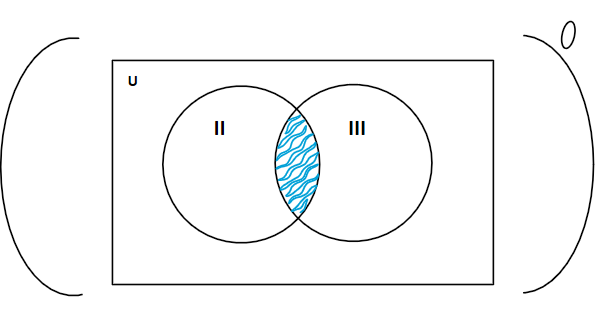
\includegraphics[width=8cm]{d/aa.png}
\caption[]{Diagrama de Venn de (II $\cap$ III)'}
\end{figure} 

\newpage

Sacando el complemento, queda el diagrama

\begin{figure}[htbp]
\centering
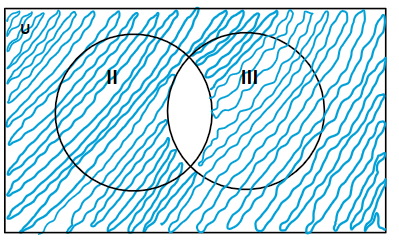
\includegraphics[width=8cm]{d/aaa.png}
\caption[]{Diagrama de Venn de (II $\cap$ III)'}
\end{figure} 

\textbf{(I $\cup$ II')'}:

\begin{figure}[htbp]
\centering
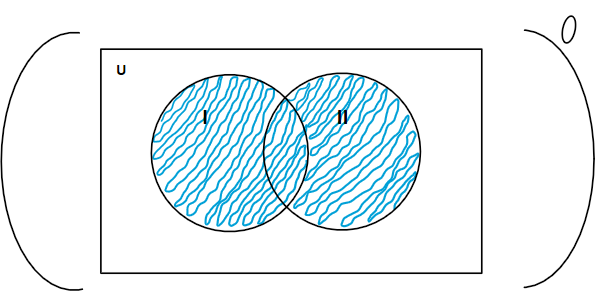
\includegraphics[width=8cm]{d/bb.png}
\caption[]{Diagrama de Venn de (I $\cup$ II')'}
\end{figure} 

Sacando el complemento, queda el diagrama

\begin{figure}[htbp]
\centering
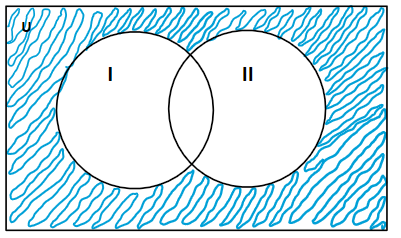
\includegraphics[width=7cm]{d/bbb.png}
\caption[]{Diagrama de Venn de (I $\cup$ II')'}
\end{figure} 

\newpage

Haciendo la intersección de ambos lados para armar (II $\cap$ III)' $\cap$ (I $\cup$ II')', quedando así el diagrama de Venn:

\begin{figure}[htbp]
\centering
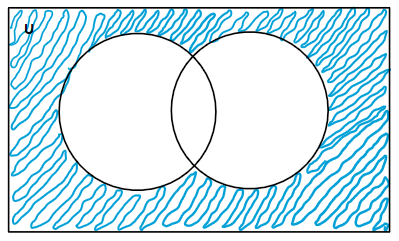
\includegraphics[width=8cm]{d/aabb.png}
\caption[]{Diagrama de Venn de (II $\cap$ III)' $\cap$ (I $\cup$ II')'}
\end{figure} 
